% 原书印刷页 34--40；第 40 页的 3.5 节开头由下一文件承接。
\sourcepage{34}
\begin{example}{3.11}
我们将算法~3.21 用于例~1.1、3.4 和~3.7 中的数据拟合问题。与例~3.7 一样，取初始点
$\mathbf{x}_0=[-1,-2,1,-1]^{\T}$，并取 $\Delta_0=1$；停止准则的参数为
$\varepsilon_1=\varepsilon_2=\varepsilon_3=10^{-8}$、$k_{\max}=200$。
算法经过 30 次迭代后停止，得到 $\mathbf{x}\simeq[-4,-5,4,-4]^{\T}$。
其表现如下图所示。与图~3.3 一样，可以看到最终阶段的收敛速度非常快。

\begin{figure}[H]
  \centering
  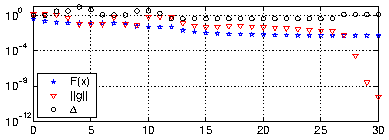
\includegraphics[width=0.68\linewidth]{assets/figures/fig-3-6.pdf}
  \setcounter{figure}{5}
  \caption{Dog Leg 法用于例~1.1 中的拟合问题。}
  \label{fig:3.6}
\end{figure}
\end{example}

上面两个例子似乎表明，Dog Leg 法远优于 Levenberg--Marquardt 法。
当最小二乘问题来自非线性方程组时，确实如此。目前，Dog Leg 法被认为是求解非线性方程组的最佳方法。

对于一般的最小二乘问题，Dog Leg 法与 L--M 法有同样的缺点：如果 $F(\mathbf{x}^*)\ne0$，
则预计最终阶段只能达到线性收敛，而且收敛缓慢。
对于给定的问题和给定的初始猜测 $\mathbf{x}_0$，无法预先判断这两种方法中哪一种更快。

\section{混合法：L--M 与拟 Newton 法}

1988 年，Madsen 提出了一种混合法，将 L--M 法与拟\setcounter{footnote}{4}\footnote{源自拉丁语：\textit{quasi} 意为“几乎”。拟 Newton 法的一般介绍见 Frandsen 等（2004）第~5~章。}
Newton 法结合起来。L--M 法在 $F(\mathbf{x}^*)=0$ 时二次收敛，否则线性收敛；
拟 Newton 法则即使在
\sourcepage{35}
$F(\mathbf{x}^*)\ne0$ 时也能超线性收敛。
迭代首先进行一系列 L--M 步。如果迭代的表现说明 $F(\mathbf{x}^*)$ 显著不为零，
就切换到拟 Newton 法，以获得更好的表现。
也可能出现迹象，说明切回 L--M 法更好，因此算法还设有相应的切换机制。

如果条件
\begin{equation}
  \norm{\mathbf{F}'(\mathbf{x})}_{\infty}<0.02\cdot F(\mathbf{x})
  \tag{3.22}\label{eq:3.22}
\end{equation}
在连续三个成功的迭代步中都成立，就切换到拟 Newton 法。
我们将这解释为一个迹象：迭代正在接近某个 $\mathbf{x}^*$，且该点满足
$\mathbf{F}'(\mathbf{x}^*)=\mathbf{0}$，而 $F(\mathbf{x}^*)$ 显著不为零。
如讨论式~\eqref{eq:3.12} 时所述，这可能导致缓慢的线性收敛。

拟 Newton 法的基础是，在当前迭代点 $\mathbf{x}$ 处有一个 Hessian 矩阵
$\mathbf{F}''(\mathbf{x})$ 的近似矩阵 $\mathbf{B}$；步向量 $\mathbf{h}_{\mathrm{qn}}$ 通过求解下式得到：
\begin{equation}
  \mathbf{B}\mathbf{h}_{\mathrm{qn}}=-\mathbf{F}'(\mathbf{x}).
  \tag{3.23}\label{eq:3.23}
\end{equation}
这是 Newton 方程~\eqref{eq:2.9a} 的近似形式。

近似矩阵 $\mathbf{B}$ 按照 BFGS 策略更新，参见 Frandsen 等（2004）第~5.10~节：
近似矩阵序列中的每一个 $\mathbf{B}$ 都是对称的（与任意 $\mathbf{F}''(\mathbf{x})$ 一样）且正定。
这保证了 $\mathbf{h}_{\mathrm{qn}}$ 是“下坡”方向，参见式~\eqref{eq:2.10}。
我们以对称正定矩阵 $\mathbf{B}_0=\mathbf{I}$ 为初始矩阵；BFGS 更新就是在当前 $\mathbf{B}$ 上加上一个秩二矩阵。
Madsen（1988）采用了 Al-Baali 和 Fletcher（1985）倡导的如下版本：
\begin{equation}
\begin{aligned}
  &\mathbf{h}:=\mathbf{x}_{\mathrm{new}}-\mathbf{x};\qquad
   \mathbf{y}:=\mathbf{J}_{\mathrm{new}}^{\T}\mathbf{J}_{\mathrm{new}}\mathbf{h}
        +(\mathbf{J}_{\mathrm{new}}-\mathbf{J})^{\T}\mathbf{f}(\mathbf{x}_{\mathrm{new}}),\\
  &\textbf{if }\mathbf{h}^{\T}\mathbf{y}>0\\
  &\qquad \mathbf{v}:=\mathbf{B}\mathbf{h};\qquad
    \mathbf{B}:=\mathbf{B}+\left(\frac{1}{\mathbf{h}^{\T}\mathbf{y}}\mathbf{y}\right)\mathbf{y}^{\T}
        -\left(\frac{1}{\mathbf{h}^{\T}\mathbf{v}}\mathbf{v}\right)\mathbf{v}^{\T}.
\end{aligned}
\tag{3.24}\label{eq:3.24}
\end{equation}
这里 $\mathbf{J}=\mathbf{J}(\mathbf{x})$，$\mathbf{J}_{\mathrm{new}}=\mathbf{J}(\mathbf{x}_{\mathrm{new}})$。
如前所述，当前的 $\mathbf{B}$ 是正定的，而且仅当 $\mathbf{h}^{\T}\mathbf{y}>0$ 时才改变它。
在这种情况下，可以证明新的 $\mathbf{B}$ 也正定。

\sourcepage{36}
拟 Newton 法在迭代的全局阶段并不稳健；不能保证它使目标函数下降。
在解 $\mathbf{x}^*$ 处有 $\mathbf{F}'(\mathbf{x}^*)=\mathbf{0}$，而 $\norm{\mathbf{F}'(\mathbf{x})}$ 的值迅速减小，
则表明最终阶段收敛良好。如果这些范数值减小得不够快，就切回 L--M 法。

算法概述如下。它调用辅助函数 \textit{LMstep} 和 \textit{QNstep}，分别实现这两种方法。

\begin{algorithmbox}{3.25}{混合法}
\label{alg:3.25}
\small
\begin{tabbing}
\qquad\=\qquad\=\qquad\=\qquad\=\qquad\=\kill
\textbf{begin}\\
\> $k:=0;\quad\mathbf{x}:=\mathbf{x}_0;\quad\mu:=\mu_0;\quad \mathbf{B}:=\mathbf{I}$
   \` $\{1^{\circ}\}$\\
\> $\mathit{found}:=(\norm{\mathbf{F}'(\mathbf{x})}_{\infty}\le\varepsilon_1);\quad
       \mathit{method}:=\text{L--M}$\\
\> \textbf{while} $(\textbf{not }\mathit{found})$ \textbf{and} $(k<k_{\max})$\\
\>\> $k:=k+1$\\
\>\> \textbf{case} $\mathit{method}$ \textbf{of}\\
\>\>\> L--M：\\
\>\>\>\> $[\mathbf{x}_{\mathrm{new}},\mathit{found},\mathit{better},\mathit{method},\ldots]
              :=\operatorname{LMstep}(\mathbf{x},\ldots)$
              \` $\{2^{\circ}\}$\\
\>\>\> Q--N：\\
\>\>\>\> $[\mathbf{x}_{\mathrm{new}},\mathit{found},\mathit{better},\mathit{method},\ldots]
              :=\operatorname{QNstep}(\mathbf{x},\mathbf{B},\ldots)$
              \` $\{2^{\circ}\}$\\
\>\> 按式~\eqref{eq:3.24} 更新 $\mathbf{B}$ \` $\{3^{\circ}\}$\\
\>\> \textbf{if} $\mathit{better}$\\
\>\>\> $\mathbf{x}:=\mathbf{x}_{\mathrm{new}}$\\
\textbf{end}
\end{tabbing}
\end{algorithmbox}

说明如下：
\begin{enumerate}[label=\(\arabic*^{\circ}\),leftmargin=2.8em]
  \item 初始化。$\mu_0$ 可由式~\eqref{eq:3.14} 确定。停止准则由式~\hyperref[eq:3.15a]{(3.15)} 给出。
  \item 省略号表示还传递 $\mathbf{f}$、$\mathbf{J}$ 等的当前值，从而不必对同一个 $\mathbf{x}$ 重复计算它们。
  \item 注意，L--M 步和拟 Newton 步都会为 Hessian 矩阵的近似提供信息。
\end{enumerate}
下面给出这两个辅助函数。

\needspace{24\baselineskip}
\sourcepage{37}
\begin{statement}{函数 3.26\quad Levenberg--Marquardt 步}
\label{fn:3.26}
\small
\[
  [\mathbf{x}_{\mathrm{new}},\mathit{found},\mathit{better},\mathit{method},\ldots]
       :=\operatorname{LMstep}(\mathbf{x},\ldots)
\]
\begin{tabbing}
\quad\=\quad\=\quad\=\quad\=\quad\=\quad\=\kill
\textbf{begin}\\
\> $\mathbf{x}_{\mathrm{new}}:=\mathbf{x};\quad\mathit{method}:=\text{L--M}$\\
\> 求解 $(\mathbf{J}(\mathbf{x})^{\T}\mathbf{J}(\mathbf{x})+\mu \mathbf{I})\mathbf{h}_{\mathrm{lm}}=-\mathbf{F}'(\mathbf{x})$\\
\> \textbf{if} $\norm{\mathbf{h}_{\mathrm{lm}}}\le\varepsilon_2(\norm{\mathbf{x}}+\varepsilon_2)$\\
\>\> $\mathit{found}:=\textbf{true}$\\
\> \textbf{else}\\
\>\> $\mathbf{x}_{\mathrm{new}}:=\mathbf{x}+\mathbf{h}_{\mathrm{lm}}$\\
\>\> $\varrho:=(F(\mathbf{x})-F(\mathbf{x}_{\mathrm{new}}))/(L(\mathbf{0})-L(\mathbf{h}_{\mathrm{lm}}))$
       \` $\{4^{\circ}\}$\\
\>\> \textbf{if} $\varrho>0$\\
\>\>\> $\mathit{better}:=\textbf{true};\quad
           \mathit{found}:=(\norm{\mathbf{F}'(\mathbf{x}_{\mathrm{new}})}_{\infty}\le\varepsilon_1)$\\
\>\>\> \textbf{if} $\norm{\mathbf{F}'(\mathbf{x}_{\mathrm{new}})}_{\infty}<0.02\cdot F(\mathbf{x}_{\mathrm{new}})$
         \` $\{5^{\circ}\}$\\
\>\>\>\> $\mathit{count}:=\mathit{count}+1$\\
\>\>\>\> \textbf{if} $\mathit{count}=3$ \` $\{6^{\circ}\}$\\
\>\>\>\>\> $\mathit{method}:=\text{Q--N}$\\
\>\>\> \textbf{else}\\
\>\>\>\> $\mathit{count}:=0$\\
\>\> \textbf{else}\\
\>\>\> $\mathit{count}:=0;\quad\mathit{better}:=\textbf{false}$\\
\textbf{end}
\end{tabbing}
\end{statement}

关于函数 \textit{LMstep} 和 \textit{QNstep}，还有以下说明：
\begin{enumerate}[label=\(\arabic*^{\circ}\),start=4,leftmargin=2.8em]
  \item 与算法~3.16 一样，增益比 $\varrho$ 还用于更新 $\mu$。
  \item 这是可能需要切换方法的迹象。参数 $\mathit{count}$ 在算法~3.25 开始时初始化为零。
  \item 式~\eqref{eq:3.22} 在连续三个迭代步中都成立，且这三步都有 $\varrho>0$，即每一步都改变了 $\mathbf{x}$。
\end{enumerate}

\needspace{24\baselineskip}
\sourcepage{38}
\begin{statement}{函数 3.27\quad 拟 Newton 步}
\label{fn:3.27}
\small
\[
  [\mathbf{x}_{\mathrm{new}},\mathit{found},\mathit{better},\mathit{method},\ldots]
       :=\operatorname{QNstep}(\mathbf{x},\mathbf{B},\ldots)
\]
\begin{tabbing}
\quad\=\quad\=\quad\=\quad\=\quad\=\kill
\textbf{begin}\\
\> $\mathbf{x}_{\mathrm{new}}:=\mathbf{x};\quad\mathit{method}:=\text{Q--N};\quad
       \mathit{better}:=\textbf{false}$\\
\> 求解 $\mathbf{B}\mathbf{h}_{\mathrm{qn}}=-\mathbf{F}'(\mathbf{x})$\\
\> \textbf{if} $\norm{\mathbf{h}_{\mathrm{qn}}}\le\varepsilon_2(\norm{\mathbf{x}}+\varepsilon_2)$\\
\>\> $\mathit{found}:=\textbf{true}$\\
\> \textbf{else}\\
\>\> \textbf{if} $\norm{\mathbf{h}_{\mathrm{qn}}}>\Delta$ \` $\{7^{\circ}\}$\\
\>\>\> $\mathbf{h}_{\mathrm{qn}}:=(\Delta/\norm{\mathbf{h}_{\mathrm{qn}}})\mathbf{h}_{\mathrm{qn}}$\\
\>\> $\mathbf{x}_{\mathrm{new}}:=\mathbf{x}+\mathbf{h}_{\mathrm{qn}}$\\
\>\> \textbf{if} $\norm{\mathbf{F}'(\mathbf{x}_{\mathrm{new}})}_{\infty}\le\varepsilon_1$
       \` $\{8^{\circ}\}$\\
\>\>\> $\mathit{found}:=\textbf{true}$\\
\>\> \textbf{else} \` $\{9^{\circ}\}$\\*
\>\>\> $\mathit{better}:=(F(\mathbf{x}_{\mathrm{new}})<F(\mathbf{x}))$ \textbf{or}\\*
\>\>\>\> $(F(\mathbf{x}_{\mathrm{new}})\le(1+\delta)F(\mathbf{x})$\\*
\>\>\>\> \textbf{and} $\norm{\mathbf{F}'(\mathbf{x}_{\mathrm{new}})}_{\infty}<\norm{\mathbf{F}'(\mathbf{x})}_{\infty})$\\
\>\>\> \textbf{if} $\norm{\mathbf{F}'(\mathbf{x}_{\mathrm{new}})}_{\infty}\ge\norm{\mathbf{F}'(\mathbf{x})}_{\infty}$
         \` $\{10^{\circ}\}$\\
\>\>\>\> $\mathit{method}:=\text{L--M}$\\
\textbf{end}
\end{tabbing}
\end{statement}

\begin{enumerate}[label=\(\arabic*^{\circ}\),start=7,leftmargin=2.8em]
  \item 我们将拟 Newton 法与信赖域方法结合起来，并对约束起作用的情形作简单处理，
        参见第~\pageref{src:15}~页及下一页。从 L--M 法切换过来时，$\Delta$ 初始化为
        \[
          \max\left\{1.5\varepsilon_2(\norm{\mathbf{x}}+\varepsilon_2),\;
                      \frac{1}{5}\norm{\mathbf{h}_{\mathrm{lm}}}\right\}.
        \]
  \item 未在伪代码中列出：用式~\eqref{eq:2.19} 更新 $\Delta$。
  \item 在算法的这一部分，我们着重于使 $\mathbf{F}'$ 更接近于零，因此允许 $F$ 的值略微增大。
        例如，可取 $\delta=\sqrt{\varepsilon_M}$，其中 $\varepsilon_M$ 是计算机的单位舍入误差。
  \item 梯度减小得不够快。
\end{enumerate}

\sourcepage{39}
\begin{example}{3.12}
注意，更新公式~\eqref{eq:3.24} 中 $\mathbf{y}$ 的计算涉及乘积
$\mathbf{J}(\mathbf{x})^{\T}\mathbf{f}(\mathbf{x}_{\mathrm{new}})$。
这意味着我们必须保存前一次的 Jacobian 矩阵。也可以在更新公式中改用
\[
  \mathbf{y}=\mathbf{F}'(\mathbf{x}_{\mathrm{new}})-\mathbf{F}'(\mathbf{x})=\mathbf{g}_{\mathrm{new}}-\mathbf{g},
\]
不过 Madsen（1988）发现，式~\eqref{eq:3.24} 的表现更好。

Madsen（1988）的拟 Newton 步没有包含信赖域处理；但在开发 immoptibox 函数
\texttt{nlshybrid} 的过程中，发现这一想法能够改善算法表现。
它减少了无效尝试 Q--N 步的次数；所谓无效尝试，是指第~$10^{\circ}$~条中的条件立即使算法返回 L--M 法。
\end{example}

\begin{example}{3.13}
对于例~3.7 和~3.8 讨论的问题，这种混合法不会优于算法~3.16。
在后一种情形中（见图~3.3），$F(\mathbf{x})\to0$，说明~$5^{\circ}$~中的切换条件永远不会满足。
在前一种情形中，$F(\mathbf{x}^*)$ 显著不为零，但是，正如例~3.7 所讨论的，
简单的 L--M 法已经具有所需的最终超线性收敛性。

为展示算法~3.25 的效率，我们考虑修正的 Rosenbrock 问题，参见 Frandsen 等（1999）例~5.5。
该问题由 $\mathbf{f}:\R^2\to\R^3$ 给出，其中
\[
  \mathbf{f}(\mathbf{x})=
  \begin{bmatrix}
    10(x_2-x_1^2)\\
    1-x_1\\
    \lambda
  \end{bmatrix},
\]
参数 $\lambda$ 可以选择。
$F(\mathbf{x})=\tfrac12\mathbf{f}(\mathbf{x})^{\T}\mathbf{f}(\mathbf{x})$ 的极小点为
$\mathbf{x}^*=[1,1]^{\T}$，且 $F(\mathbf{x}^*)=\tfrac12\lambda^2$。

下面给出若干 $\lambda$ 值下算法~3.16 和~3.25 的结果。
在所有情形中，都取 $\mathbf{x}_0=[-1.2,1]^{\T}$；初始阻尼参数 $\mu_0$ 由
式~\eqref{eq:3.14} 定义，其中 $\tau=10^{-3}$；停止准则~\hyperref[eq:3.15a]{(3.15)} 中取
$(\varepsilon_1,\varepsilon_2,k_{\max})=(10^{-10},10^{-14},200)$。

在前两种情形中，$\lambda$ 太小，不会真正影响迭代；但当 $\lambda$ 较大时，
可以看到混合法远优于简单的 Levenberg--Marquardt 算法，尤其是在所获得的精度方面。

图~\ref{fig:3.7} 展示了 $\lambda=10^4$ 时这两种算法的表现。

\sourcepage{40}
\begin{center}
\small
\begin{tabular}{|c|rr|rr|}
  \cline{2-5}
  \multicolumn{1}{c|}{} & \multicolumn{2}{c|}{算法 3.16} & \multicolumn{2}{c|}{算法 3.25}\\
  \hline
  $\lambda$ & 迭代步数 & $\norm{\mathbf{x}-\mathbf{x}^*}$ & 迭代步数 & $\norm{\mathbf{x}-\mathbf{x}^*}$\\
  \hline
  $0$       & 17 & $2.78\times10^{-12}$ & 17 & $2.78\times10^{-12}$\\
  $10^{-5}$ & 17 & $2.78\times10^{-12}$ & 17 & $2.78\times10^{-12}$\\
  $1$       & 24 & $1.69\times10^{-9}$  & 19 & $2.23\times10^{-14}$\\
  $10^2$    & 23 & $5.87\times10^{-7}$  & 22 & $3.16\times10^{-12}$\\
  $10^4$    & 23 & $2.37\times10^{-4}$  & 22 & $3.16\times10^{-12}$\\
  \hline
\end{tabular}
\end{center}

\begin{figure}[H]
  \centering
  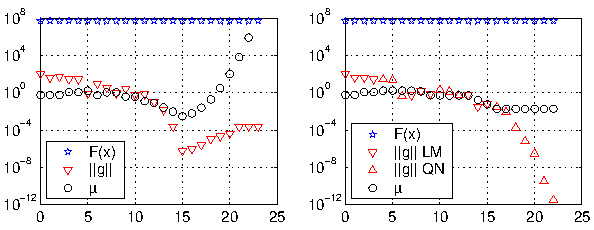
\includegraphics[width=0.96\linewidth]{assets/figures/fig-3-7.pdf}
  \setcounter{figure}{6}
  \caption{Levenberg--Marquardt 法（左）与混合法（右）。}
  \label{fig:3.7}
\end{figure}

使用 L--M 法时，第 15 步之后的所有步骤都未能改善目标函数；
$\mu$ 迅速增大，第 23 步满足停止准则~\eqref{eq:3.15b}，迭代因而终止。

使用混合法时，分别从第 5、11 和 17 步开始，多次尝试使用拟 Newton 法。
最后一次尝试成功，经过 22 步后，迭代由式~\eqref{eq:3.15a} 停止。
\end{example}
